\chapter{Singular Value Decomposition}
\label{chap:SingularValueDecomposition}

Recall that a line through the origin in $\Re^n$ is 
$\set{r\cdot \vec{v}\suchthat r\in\Re}$. 
One of the defining properties of a linear map is that 
$h(r\cdot\vec{v})=r\cdot h(\vec{v})$.
So the action of $h$ on any 
line through the origin
is determined by the action
of $h$ on any nonzero vector in that line.

For instance consider the line~$y=2x$ in the plane.
\begin{equation*}
  \set{r\cdot\colvec{1 \\ 2}\suchthat r\in\Re}
\end{equation*}
If $\map{t}{\Re^2}{\Re^2}$ is represented by the matrix
\begin{equation*}
  \rep{t}{\stdbasis_2,\stdbasis_2}
  =
  \begin{mat}
    1 &2 \\
    3 &4
  \end{mat}
\end{equation*}
then here is the effect of $t$ on one vector in the line
(calculating with the vector on the left $\vec{v}T$).
\begin{equation*}
  \vec{v}=\colvec{1 \\ 2}\mapsunder{t}\colvec{7 \\ 10}
\end{equation*}
The map $t$ has twice the effect on $2\vec{v}$, three times the
effect on $3\vec{v}$, etc.
\begin{equation*}
  \colvec{2 \\ 4}\mapsunder{t}\colvec{14 \\ 20}
  \qquad
  \colvec{-3 \\ -6}\mapsunder{t}\colvec{-21 \\ -30}
  \qquad
  \colvec{r \\ 2r}\mapsunder{t}\colvec{7r \\ 10r}
\end{equation*}
So this condition in the definition of linear map imposes a simple
uniformity on its action on lines through the origin.




\section{Unit circle}
Consider transformations of the plane $\Re^2$.
Because of $t(r\cdot\vec{v})=r\cdot t(\vec{v})$,
one way to describe a transformation's action is to pick 
a set containing one nonzero vector from each line through the origin
and describe where the transformation maps those elements.

A natural set that contains one nonzero element from each line through the
origin is the upper half unit circle.
\begin{sageoutput}
runfile("plot_action.sage")
p = plot_circle_action(1,0,0,1) 
p.set_axes_range(-1.5, 1.5, -0.5, 1.5) 
p.save("graphics/svd000.pdf")
\end{sageoutput}
\begin{sagesilent}
load("plot_action.sage")
p = plot_circle_action(1,0,0,1) 
p.set_axes_range(-1.5, 1.5, -0.5, 1.5) 
p.save("graphics/svd000.pdf")
\end{sagesilent}
\begin{equation*}
  U=\set{\colvec{x \\ y}
         \suchthat 
         \text{$x=\cos(t)$, $y=\sin(t)$, $0\leq t<\pi$}}
  \qquad
  \vcenteredhbox{\includegraphics{graphics/svd000.pdf}}  
\end{equation*}
The above 
graph came from  using a routine that draws the effect of a transformation 
on the unit circle
and then specifying the identity transformation.
\begin{sageoutput}
runfile("plot_action.sage")
p = plot_circle_action(1,0,0,1)  # identity matrix
p.set_axes_range(-1.5, 1.5, -0.5, 1.5) 
p.save("graphics/svd000.pdf")
\end{sageoutput}
Its source code is 
at the end of this chapter but in short 
\inlinecode{plot_circle_action(a,b,c,d)}
multiplies points on 
the unit circle by this matrix.
\begin{equation*}
  \begin{mat}
    a &b \\
    c &d
  \end{mat}
\end{equation*}
The colors are for the 
before and after pictures below.

Here is the effect of 
the transformation 
\begin{equation*}
  \colvec{x \\ y} \mapsto \colvec{2x \\ y}
\end{equation*}
that doubles the $x$~component of input vectors. 
It shows before and after, the upper half circle domain
and the output codomain.\footnote{noterightmult}
\begin{sageoutput}[d,0,4;d,5,7]
runfile("plot_action.sage")
q = plot_circle_action(1,0,0,1) 
q.set_axes_range(-2, 2, -1, 2) 
q.save("graphics/svd001a.pdf")
p = plot_circle_action(2,0,0,1) 
p.set_axes_range(-2, 2, -1, 2) 
p.save("graphics/svd001b.pdf")
\end{sageoutput}
\begin{sagesilent}
load("plot_action.sage")
q = plot_circle_action(1,0,0,1) 
q.set_axes_range(-2, 2, -1, 2) 
q.save("graphics/svd001a.pdf")
p = plot_circle_action(2,0,0,1) 
p.set_axes_range(-2, 2, -1, 2) 
p.save("graphics/svd001b.pdf")
\end{sagesilent}
\begin{equation*}
  \vcenteredhbox{\includegraphics{graphics/svd001a.pdf}}
  \quad\mapsunder{\big (\begin{smallmatrix} 2 &0 \\ 0 &1 \end{smallmatrix}\big )}\quad
  \vcenteredhbox{\includegraphics{graphics/svd001b.pdf}}
\end{equation*}

The next before and after picture shows
the effect of the transformation 
\begin{equation*}
  \colvec{x \\ y} \mapsto \colvec{-x \\ 3y}
\end{equation*}
that triples the $y$~component and multiplies the 
$x$~component by $-1$. 
\begin{sageoutput}[d,0,4;d,5,7]
runfile("plot_action.sage")
q = plot_circle_action(1,0,0,1) 
q.set_axes_range(-2, 2, -4, 4) 
q.save("graphics/svd002a.pdf")
p = plot_circle_action(-1,0,0,3) 
p.set_axes_range(-2, 2, -4, 4) 
p.save("graphics/svd002b.pdf")
\end{sageoutput}
\begin{sagesilent}
load("plot_action.sage")
q = plot_circle_action(1,0,0,1) 
q.set_axes_range(-2, 2, -4, 4) 
q.save("graphics/svd002a.pdf")
p = plot_circle_action(-1,0,0,3) 
p.set_axes_range(-2, 2, -4, 4) 
p.save("graphics/svd002b.pdf")
\end{sagesilent}
\begin{equation*}
  \vcenteredhbox{\includegraphics{graphics/svd002a.pdf}}
  \quad\mapsunder{\big (\begin{smallmatrix} -1 &0 \\ 0 &3 \end{smallmatrix}\big )}\quad
  \vcenteredhbox{\includegraphics{graphics/svd002b.pdf}}
\end{equation*}
Now the colors come in.
The input circle moves 
counterclockwise from red to orange, then to green, blue, indigo, and 
finally to violet.
But the output does the opposite: to move from red to violet you
move clockwise.
This transformation changes the \textit{orientation} 
(or \textit{sense}) of the curve. 

The next transformation is a skew.
\begin{equation*}
  \colvec{x \\ y} \mapsto \colvec{x+2y \\ y}
\end{equation*}
The output's first component is affected
by the input vector's distance from the $y$-axis.
\begin{sageoutput}[d,0,4;d,5,7]
runfile("plot_action.sage")
q = plot_circle_action(1,0,0,1) 
q.set_axes_range(-2, 3, -1, 2) 
q.save("graphics/svd003a.pdf")
p = plot_circle_action(1,0,2,1) 
p.set_axes_range(-2, 3, -1, 2) 
p.save("graphics/svd003b.pdf")
\end{sageoutput}
\begin{sagesilent}
load("plot_action.sage")
q = plot_circle_action(1,0,0,1) 
q.set_axes_range(-2, 3, -1, 2) 
q.save("graphics/svd003a.pdf")
p = plot_circle_action(1,0,2,1) 
p.set_axes_range(-2, 3, -1, 2) 
p.save("graphics/svd003b.pdf")
\end{sagesilent}
\begin{equation*}
  \vcenteredhbox{\includegraphics{graphics/svd003a.pdf}}
  \quad\mapsunder{\big (\begin{smallmatrix} 1 &0 \\ 2 &1 \end{smallmatrix}\big )}\quad
  \vcenteredhbox{\includegraphics{graphics/svd003b.pdf}}
\end{equation*}

Here is another skew.
In this case the output's 
second component is affected by the input's distance from 
the $x$-axis.
\begin{sageoutput}[d,0,4;d,5,7]
runfile("plot_action.sage")
q = plot_circle_action(1,0,0,1) 
q.set_axes_range(-2, 2, -2, 2) 
q.save("graphics/svd004a.pdf")
p = plot_circle_action(1,1/2,0,1) 
p.set_axes_range(-2, 2, -2, 2) 
p.save("graphics/svd004b.pdf")
\end{sageoutput}
\begin{sagesilent}
load("plot_action.sage")
q = plot_circle_action(1,0,0,1) 
q.set_axes_range(-2, 2, -2, 2) 
q.save("graphics/svd004a.pdf")
p = plot_circle_action(1,1/2,0,1) 
p.set_axes_range(-2, 2, -2, 2) 
p.save("graphics/svd004b.pdf")
\end{sagesilent}
\begin{equation*}
  \vcenteredhbox{\includegraphics{graphics/svd004a.pdf}}
  \quad\mapsunder{\big (\begin{smallmatrix} 1 &1/2 \\ 0 &1 \end{smallmatrix}\big )}\quad
  \vcenteredhbox{\includegraphics{graphics/svd004b.pdf}}
\end{equation*}

And here is a generic transformation.
It changes orientation also.
\begin{sageoutput}[d,0,4;d,5,7]
runfile("plot_action.sage")
q = plot_circle_action(1,0,0,1) 
q.set_axes_range(-2, 4, -3, 6) 
q.save("graphics/svd005a.pdf")
p = plot_circle_action(1,2,3,4) 
p.set_axes_range(-2, 4, -3, 6) 
p.save("graphics/svd005b.pdf")
\end{sageoutput}
\begin{sagesilent}
load("plot_action.sage")
q = plot_circle_action(1,0,0,1) 
q.set_axes_range(-2, 4, -3, 6) 
q.save("graphics/svd005a.pdf",figsize=3)
p = plot_circle_action(1,2,3,4) 
p.set_axes_range(-2, 4, -3, 6) 
p.save("graphics/svd005b.pdf",figsize=3)
\end{sagesilent}
\begin{equation*}
  \vcenteredhbox{\includegraphics{graphics/svd005a.pdf}}
  \quad\mapsunder{\big (\begin{smallmatrix} 1 &2 \\ 3 &4 \end{smallmatrix}\big )}\quad
  \vcenteredhbox{\includegraphics{graphics/svd005b.pdf}}
\end{equation*}



\section{SVD}
The above pictures show the unit circle mapping to ellipses.
Recall that in $\Re^2$ an ellipse has a \textit{major axis}, 
the longer one, and a 
\textit{minor axis}.\footnote{If the two axes have the same length 
then the ellipse is a circle.
If one axis has length zero then the ellipse is a line segment 
and if both have length zero then it is a point.}
Write $\sigma_1$ for the length of the semi-major axis, 
the distance from the center to the furthest-away point on the ellipse,
and write $\sigma_2$ for the length of the semi-minor axis.
\begin{sageoutput}[d,0,4]
plot.options['axes_pad'] = 0.5
plot.options['fontsize'] = 5
plot.options['aspect_ratio'] = 1
sigma_1=3
sigma_2=1
E = ellipse((0,0), sigma_1, sigma_2)
E.save("graphics/svd100.pdf",figsize=4)
\end{sageoutput}
\begin{sagesilent}
plot.options['axes_pad'] = 0.5
plot.options['fontsize'] = 5
plot.options['aspect_ratio'] = 1
plot.options['figsize'] = 1
sigma_1=3
sigma_2=1
E = ellipse((0,0), sigma_1, sigma_2)
# E.save("graphics/svd100.pdf", axes_pad=0.075, dpi=1200, fontsize=7, ticks=([-3,-2,-1,1,2,3],[-1,1]), figsize=1.5)
E.save("graphics/svd100.pdf", axes_pad=0.075, figsize=4)
\end{sagesilent}
\begin{center}
  \includegraphics{graphics/svd100.pdf}
\end{center}
In an ellipse the two axes are orthogonal.
In the above graph the major axis lies along the $x$-axis while the
minor axis lies along the $y$-axis.

Under any linear map $\map{t}{\Re^n}{\Re^m}$ the 
unit sphere maps to a hyperellipse.
This is a version of the \textit{Singular Value Decomposition} of
matrices:
for any linear map $\map{t}{\Re^m}{\Re^n}$ there are bases
$B=\sequence{\vec{\beta}_1,\ldots,\vec{\beta}_m}$ for the domain and
$D=\sequence{\vec{\delta}_1,\ldots,\vec{\delta}_n}$ for the codomain
such that $t(\vec{\beta}_i)=\sigma_i\vec{\delta}_i$, where the
\textit{singular values}
$\sigma_i$ are scalars.
The next section sketches a proof
but we first illustrate this result by using an example matrix.
\Sage{} will find the two bases $B$ and~$D$ and will picture how the 
vectors $\vec{\beta}_i$ 
are mapped to the $\sigma_i\vec{\delta}_i$.

So consider again the generic matrix.
Here is its action again, this time shown
on a full circle.
\begin{sageoutput}[d,0,4;d,5,7]
runfile("plot_action.sage")
q = plot_circle_action(1,0,0,1,full_circle=True) 
q.set_axes_range(-2, 2, -5, 6) 
q.save("graphics/svd101a.pdf")
p = plot_circle_action(1,2,3,4,full_circle=True) 
p.set_axes_range(-4, 4, -5, 6) 
p.save("graphics/svd101b.pdf")
\end{sageoutput}
\begin{sagesilent}
load("plot_action.sage")
q = plot_circle_action(1,0,0,1,full_circle=True) 
q.set_axes_range(-2, 2, -5, 6) 
q.save("graphics/svd101a.pdf")
p = plot_circle_action(1,2,3,4,full_circle=True) 
p.set_axes_range(-4, 4, -5, 6) 
p.save("graphics/svd101b.pdf")
\end{sagesilent}
\begin{equation*}
  \vcenteredhbox{\includegraphics{graphics/svd101a.pdf}}
  \quad\mapsunder{\big (\begin{smallmatrix} 1 &2 \\ 3 &4 \end{smallmatrix}\big )}\quad
  \vcenteredhbox{\includegraphics{graphics/svd101b.pdf}}
  \tag{$*$}
\end{equation*}
\Sage{} will find the SVD of this example matrix.
\begin{sageoutput}
M = matrix(RDF, [[1, 2], [3, 4]])
U,Sigma,V = M.SVD()
U
Sigma
V
U*Sigma*(V.transpose())
\end{sageoutput}
\noindent 
The Singular Value Decomposition has $M$ as the product of
three matrices, $U\Sigma\trans{V}$.
The basis vectors $\vec{\beta}_1$, $\vec{\beta}_2$, $\vec{\delta}_1$, 
and~$\vec{\delta}_2$ are the columns of $U$ and~$V$. 
The singular values are the diagonal entries of~$\Sigma$.
\Sage{} will plot the effect of the transformation
on the basis vectors for the domain so we can compare those with the
basis vectors for the codomain.
\begin{sageoutput}[d,0,2;d,6,10]
M = matrix(RDF, [[1, 2], [3, 4]])
U,Sigma,V = M.SVD()
beta_1 = vector(RDF, [U[0][0], U[1][0]])
beta_2 = vector(RDF, [U[0][1], U[1][1]])
delta_1 = vector(RDF, [V[0][0], V[1][0]])
delta_2 = vector(RDF, [V[0][1], V[1][1]])
plot.options['axes_pad'] = 0.05
plot.options['fontsize'] = 7
plot.options['aspect_ratio'] = 1
C = circle((0,0), 1)
P = C + plot(beta_1) + plot(beta_2)
P.save("graphics/svd102a.pdf",figsize=2)
image_color=Color(1,0.5,0.5)   # color for t(beta_1), t(beta_2)
Q = C + plot(beta_1*M, width=3, color=image_color) 
Q = Q + plot(delta_1,width=1.4, color='blue') 
Q = Q + plot(beta_2*M,width=3, color=image_color) 
Q = Q + plot(delta_2,width=1.4, color='blue')
Q.save("graphics/svd102b.pdf")
\end{sageoutput}
\begin{sagesilent}
M = matrix(RDF, [[1, 2], [3, 4]])
U,Sigma,V = M.SVD()
beta_1 = vector(RDF, [U[0][0], U[1][0]])
beta_2 = vector(RDF, [U[0][1], U[1][1]])
delta_1 = vector(RDF, [V[0][0], V[1][0]])
delta_2 = vector(RDF, [V[0][1], V[1][1]])
plot.options['axes_pad'] = 0.05
plot.options['fontsize'] = 7
plot.options['aspect_ratio'] = 1
arrowsize = 2
C = circle((0,0), 1)
P = C + plot(beta_1,arrowsize=arrowsize) + plot(beta_2,arrowsize=arrowsize)
P.save("graphics/svd102a.pdf", figsize=2, axes_pad=0.05)
image_color=Color(1,0.5,0.5)   # color for t(beta_1), t(beta_2)
Q = C + plot(beta_1*M, width=3, arrowsize=arrowsize, color=image_color) 
Q = Q + plot(delta_1,width=1.4, arrowsize=arrowsize,color='blue') 
Q = Q + plot(beta_2*M,width=3, arrowsize=arrowsize,color=image_color) 
Q = Q + plot(delta_2,width=1.4, arrowsize=arrowsize,color='blue')
Q.save("graphics/svd102b.pdf", figsize=4.467, axes_pad=0.05)
\end{sagesilent}
In the picture below the domain's 
blue $\vec{\beta}$'s on the left map to the codomain's light red 
$t(\vec{\beta})$'s on the right.
Also on the right, in blue, are the $\vec{\delta}$'s.
The red $t(\vec{\beta}_1)$ does look to be about $5.5$ times $\vec{\delta}_1$,
and $t(\vec{\beta}_2)$ does look something like $0.4$ times~$\vec{\delta}_2$. 
\begin{equation*}
  % \setlength{\fboxsep}{0in} % used to set box heights by eye; surrounded each picture env with a fbox
  \setlength{\unitlength}{1in}
  \begin{picture}(1.35,1.35)
    \put(0,1.825){\includegraphics{graphics/svd102a.pdf}}
    \put(.3,1.9){\scriptsize $\vec{\beta}_1$}
    \put(0,2.7){\scriptsize $\vec{\beta}_2$}
  \end{picture}
  \quad
  \raisebox{2.65in}{$\mapsunder{\big (\begin{smallmatrix} 1 &2 \\ 3 &4 \end{smallmatrix}\big )}$}
  \qquad
  \begin{picture}(2.45,3.15)
    \put(0,0){\includegraphics{graphics/svd102b.pdf}}
    \put(1.25,2){\scriptsize $\vec{\delta}_1$}
    \put(2.3,2.1){\scriptsize $\vec{\delta}_2$}
  \end{picture}
  \tag*{\raisebox{2.5in}{($**$)}}
\end{equation*}
Note also that the two bases are \textit{orthonormal}\Dash the unit circles help
us see that the bases are comprised of unit vectors and further,
the two members of each basis are orthogonal.

Compare this diagram to the one before it 
labeled~($*$), which shows the effect of the matrix
on the unit circle.
We used the whole circle in~($*$) to spotlight the ellipse and 
to make clearer that in~($**$)
the longest red vector is a
semi-major axis of that ellipse and the shortest red vector is a 
semi-minor axis.



\section{Proof sketch}

\textit{This argument, 
adapted from \cite{BlankKrikorianSpring89},
is a sketch because it uses results that a typical reader has only 
seen in a less general version and because it relies on material from the
book that is optional.
In addition, we'll consider only the case of a nonsingular matrix and map;
it shows the main idea, which is the point of a sketch.}

Consider an~$\nbyn{n}$ matrix~$T$ that is nonsingular, and the
nonsingular transformation~$\map{t}{\Re^n}{\Re^n}$ represented by
$T$ with respect to the standard bases.

Recall the Extreme Value Theorem from Calculus~I: for a continuous
function~$f$, if $D\subset \Re$ is a closed and bounded set then
the image $f(D)$ is also a closed and bounded 
set (see \cite{wiki:ExtremeValueThm}).
A generalization of that result gives that because the unit sphere in $\Re^n$
is closed and bounded then its image under~$t$ is closed and bounded.
Although we won't prove this, the image is an ellipsoid
so we will call it that. 

Because the ellipsoid is closed and bounded it has a point furthest from the
origin.
Let $\vec{w}$ be a vector extending from the origin to that furthest point.
Let $\vec{v}$ be the member of the unit sphere that maps to $\vec{w}$.
Let $P$ be the plane that touches the sphere only at the endpoint of $\vec{v}$.
Let $Q$ be the image of $P$ under~$t$.
Since $t$ is one-to-one, $Q$ touches the ellipsoid only at~$\vec{w}$.
\begin{center}
  \includegraphics{asy/ellipsoid1.pdf}
\end{center}

The tangent plane~$P$ has the property that 
the set of vectors whose bodies lie in~$P$
are the set of vectors perpendicular to $\vec{v}$.
That is, if in the picture above we slide $P$ along the vector~$\vec{v}$ to
the origin then we clearly have the subspace of $\Re^n$ of vectors perpendicular
to~$\vec{v}$.
This subspace has dimension~$n-1$. 
We will argue below 
that if we similarly slide $Q$ to the origin then we have the
set of vectors perpendicular to~$\vec{w}$.
With that we will have an argument by induction: we start constructing the 
bases~$B$ and~$D$ by taking $\vec{\beta}_1$ to be~$\vec{v}$, taking
$\sigma_1$ to be the length $\norm{\vec{w}}$, and taking
$\vec{\delta}_1$ to be $\vec{w}/\norm{\vec{w}}$.
Then we proceed by considering the restriction of $t$ to~$P$.

So consider~$Q$.
First observe that there is a unique plane that touches the ellipsoid
only at~$\vec{w}$ since if there were another then its inverse image
under $t$
would be a second plane, besides~$P$, 
that touches the sphere only at~$\vec{v}$, which is impossible.
To see that $Q$ is perpendicular to~$\vec{w}$ consider a sphere
centered at the origin whose radius is $\norm{\vec{w}}$.
This sphere has a plane tangent at the endpoint of~$\vec{w}$, 
which is perpendicular
to $\vec{w}$.
Because $\vec{w}$ ends at a point on the ellipsoid furthest from the origin,
the ellipsoid is entirely contained in the sphere, so this plane touches
the ellipsoid only at~$\vec{w}$.
Therefore, from the second sentence of this paragraph, this plane is~$Q$. 
That ends the argument.



\section{Matrix factorization}

We can express those geometric ideas in an algebraic form
(for a proof see \cite{TrefethenBau97}).

The \textit{singular value decomposition} of an $\nbym{m}{n}$ matrix~$A$
is a factorization $A=U\Sigma \trans{V}$.
The $\nbym{m}{n}$ matrix $\Sigma$ 
is all zeroes except for diagonal entries, the singular values, 
$\sigma_1\geq \sigma_2 \geq \cdots \geq \sigma_r> 0$ where $r$ is the
rank of~$A$.
The $\nbyn{m}$ matrix~$U$ and the $\nbyn{n}$ matrix~$V$ are unitary, meaning
that their columns form an orthogonal basis of unit vectors, the left and 
right \textit{singular vectors} for~$A$, respectively. 
\begin{sageoutput}
M = matrix(RDF, [[0, 1, 2], [3, 4, 5]])
U,Sigma,V = M.SVD()
U
Sigma
V  
\end{sageoutput}
% The number of singular values is the rank of the matrix.
% Here \Sage{} gets a $\sigma_2$ that is not quite zero because of numerical 
% issues. 
% \begin{sageoutput}
% M = matrix(RDF, [[0, 1, 2], [0, 2, 4]])
% U,Sigma,V = M.SVD()
% U
% Sigma
% V  
% \end{sageoutput}

The product $U\Sigma\trans{V}$ simplifies.
To see how,
consider the case where all three matrices are $\nbyn{2}$.
Write $\vec{u}_1$, $\vec{u}_2$ for the columns of~$U$
and $\vec{v}_1$, $\vec{v_2}$ for the columns of~$V$,
so that the rows of $\trans{V}$ are $\trans{\vec{v}}_1$ and
$\trans{\vec{v}}_2$.
\begin{align*}
  U\Sigma \trans{V}
  &=
  \begin{mat}
    \vec{u}_1 &\vec{u}_2
  \end{mat}
  \begin{mat}
    \sigma_1 &0 \\
    0        &\sigma_2
  \end{mat}
  \begin{mat}
    \trans{\vec{v}}_1 \\[.75ex]
    \trans{\vec{v}}_2
  \end{mat}             \\[.5ex]
  &=
  \begin{mat}
    \vec{u}_1 &\vec{u}_2
  \end{mat}
  \begin{mat}
    \sigma_1 &0 \\
    0        &0
  \end{mat}
  \begin{mat}
    \trans{\vec{v}}_1 \\[.75ex]
    \trans{\vec{v}}_2
  \end{mat}             
  +
  \begin{mat}
    \vec{u}_1 &\vec{u}_2
  \end{mat}
  \begin{mat}
    0        &0 \\
    0        &\sigma_2
  \end{mat}
  \begin{mat}
    \trans{\vec{v}}_1 \\[.75ex]
    \trans{\vec{v}}_2
  \end{mat}             \\[.5ex]
  &=
  \sigma_1\cdot
  \begin{mat}
    \vec{u}_1 &\vec{u}_2
  \end{mat}
  \begin{mat}
    1 &0 \\
    0 &0
  \end{mat}
  \begin{mat}
    \trans{\vec{v}}_1 \\[.75ex]
    \trans{\vec{v}}_2
  \end{mat}             
  +
  \sigma_2\cdot 
  \begin{mat}
    \vec{u}_1 &\vec{u}_2
  \end{mat}
  \begin{mat}
    0        &0 \\
    0        &1
  \end{mat}
  \begin{mat}
    \trans{\vec{v}}_1 \\[.75ex]
    \trans{\vec{v}}_2
  \end{mat}
  \tag{$*{*}*$}
\end{align*}
In the first term,
right multiplication by the $1,1$~unit matrix picks out the first column of
$U$, and left multiplication by the $1,1$~unit matrix picks out first row of
$V$ so those are the only parts that remain after the product.
In short, we get this.
\begin{equation*}
  \begin{mat}
    u_{1,1} &u_{1,2} \\
    u_{2,1} &u_{2,2}
  \end{mat}
  \begin{mat}
    1 &0 \\
    0 &0
  \end{mat}
  \begin{mat}
    v_{1,1} &v_{2,1} \\
    v_{1,2} &v_{2,2}
  \end{mat}
  =
  \begin{mat}
    u_{1,1}v_{1,1} &u_{1,1}v_{2,1} \\
    u_{2,1}v_{1,1} &u_{2,1}v_{2,1}
  \end{mat}
  =\vec{u}_1\trans{\vec{v}}_1
\end{equation*}
Thus, equation~($*{*}*$) simplifies to
$U\Sigma \trans{V}=\sigma_1\cdot\vec{u}_1\trans{\vec{v}}_1
   +\sigma_2\cdot\vec{u}_2\trans{\vec{v}}_2$.
Cases other than~$\nbyn{2}$ simplify in the same way.



\section{Application: data compression}

We can write any matrix as a sum
$M=\sigma_1\cdot\vec{u}_1\trans{\vec{v}}_1
   +\sigma_2\cdot\vec{u}_2\trans{\vec{v}}_2
   +\cdots$
where the vectors have unit size and the $\sigma_i$'s decrease in size.

Suppose that the matrix is $\nbyn{n}$.
To store or transmit it we need to work with $n^2$ real numbers.
For instance, if $n=500$ then we have $50^2=250\,000$~reals.
To express the matrix as a sum, 
each term requires 
$n$~real numbers for $\vec{u}_i$, another $n$ reals for~$\vec{v}_i$, and one
more real for $\sigma_i$.
So keeping all the terms would require $500*(2*500+1)=500\,500$~reals,
which is twice the data of the original matrix.

But if you keep only some of the terms, say the first $50$ of them, then
you would save:~$50\cdot (2n+1)=50\,050$, which is about $20\%$ of the
$500^2$~size of the full matrix.
Thus, if you have data as a matrix then you can hope to compress it
with that summation formula by dropping terms with small $\sigma$'s.  
The issue is whether you lose too much information by only 
retaining the information associated with some of the singular values.

To illustrate that you can succeed in retaining at least some aspects of data
we will do image compression.
Meet Lenna.
This top third of a pinup is a standard test image
\cite{wiki:Lenna}.
\begin{center}
  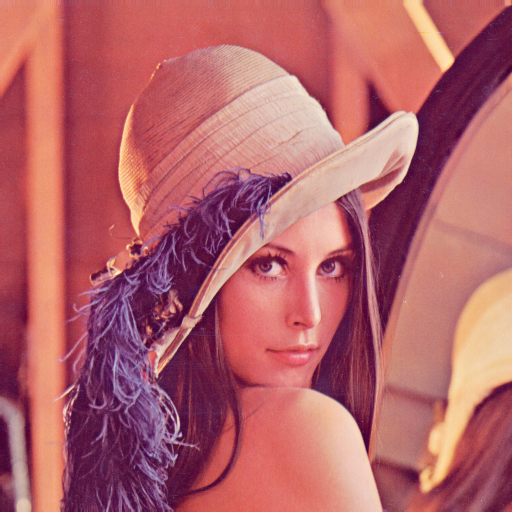
\includegraphics[width=.95\textwidth]{Lenna.png} % from http://en.wikipedia.org/wiki/File:Lenna.png
\end{center}

The code we will use is in the \inlinecode{img_squeeze} routine 
listed at the end of this chapter.
The code breaks the picture into three matrices, for the red data, the 
green data, and the blue data.
In that code we have a peek at the eight largest singular
values in the red matrix:
  $93233.7882139$, 
  $11193.1186308$, 
  $8660.12549856$, 
  $7054.38662024$, 
  $5916.89456484$, 
  $5742.14618029$, 
  $4125.16604075$, and
  $3879.15303685$.
We retain the terms for the largest $10\%$ of the singular values. 
The code reports that
the singular value where we make that cutoff is $606.389279688$.
It also gives the eight smallest:
  $0.547288023466$, 
  $0.470266870056$, 
  $0.1988515109$, 
with five more that are so small they are essentially 
zero.\footnote{These are four values of 
$1.024\,723\,452\,83\protect\times 10^{-11}$
and one of $2.325\,339\,864\,91\protect\times 10^{-12}$.}
% \begin{lstlisting}
% sigma_RD 0 = 93233.7882139
% sigma_RD 1 = 11193.1186308
% sigma_RD 2 = 8660.12549856
% sigma_RD 3 = 7054.38662024
% sigma_RD 4 = 5916.89456484
% sigma_RD 5 = 5742.14618029
% sigma_RD 6 = 4125.16604075
% sigma_RD 7 = 3879.15303685
%   :
% sigma_RD 51 = 606.389279688
%   :
% sigma_RD 504 = 0.547288023466
% sigma_RD 505 = 0.470266870056
% sigma_RD 506 = 0.1988515109
% sigma_RD 507 = 1.02472345283e-11
% sigma_RD 508 = 1.02472345283e-11
% sigma_RD 509 = 1.02472345283e-11
% sigma_RD 510 = 1.02472345283e-11
% sigma_RD 511 = 2.32533986491e-12  
% \end{lstlisting}
The large singular values are much larger than the small singular values,
even setting aside the ones at the end
that are zero except for numerical issues.

We want to see how badly the image degrades for various cutoffs.
The code below sets the cutoff at $0.10$.
This image is $\nbyn{512}$  so that will sum the terms associated
with the first $51$ singular 
values.
\begin{lstlisting}
sage: runfile("img_squeeze.sage")                                 
sage: img_squeeze("Lenna.png", "Lenna_squeezed.png", 0.10)
\end{lstlisting}
Below is the squeezed image.
\begin{center}
  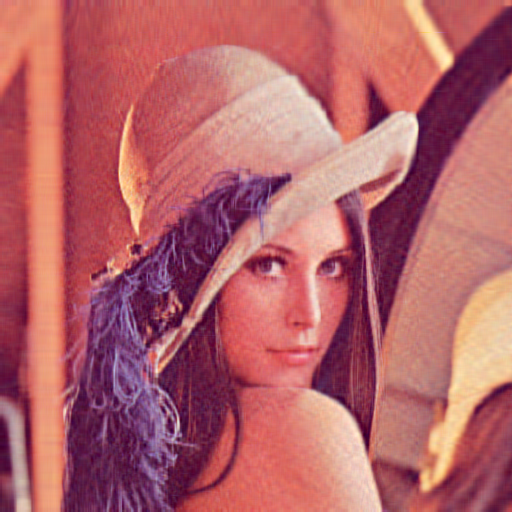
\includegraphics[width=.95\textwidth]{Lenna_squeezed.png}
\end{center}
It definitely shows loss.
The colors are not as good, the edges are not sharp, and there are 
a few artifacts, including a horizontal line across the top of 
Lenna's forehead and another halfway up her hat.
But certainly the image is entirely recognizable.

Where the image is $\nbyn{n}$, every additional term in the summation
adds to the storage and transmission requirements by about $2n$ reals.
The original image requires $n^2$ reals so we want to choose a cutoff value 
less than $0.50$.
The above image with a cutoff of $0.10$ has the advantage is that it needs 
only $20\%$ of the storage
and transmission requirements of the original image
but its quality may not be acceptable.
That is, selecting a cutoff parameter is an engineering decision where
on a fidelity versus resource-consumption continuum 
you choose a value appropriate for your application.
 
Experimenting with percentage value shows that setting
the cutoff parameter to $0.20$ is enough to make the output image hard to tell
from the original.
For a final contrast, below we use this cutoff on the picture of Suzy 
from this manual's cover.
On the left is the original image
and on the right it is squeezed using $0.20$.
\begin{center}
  \vcenteredhbox{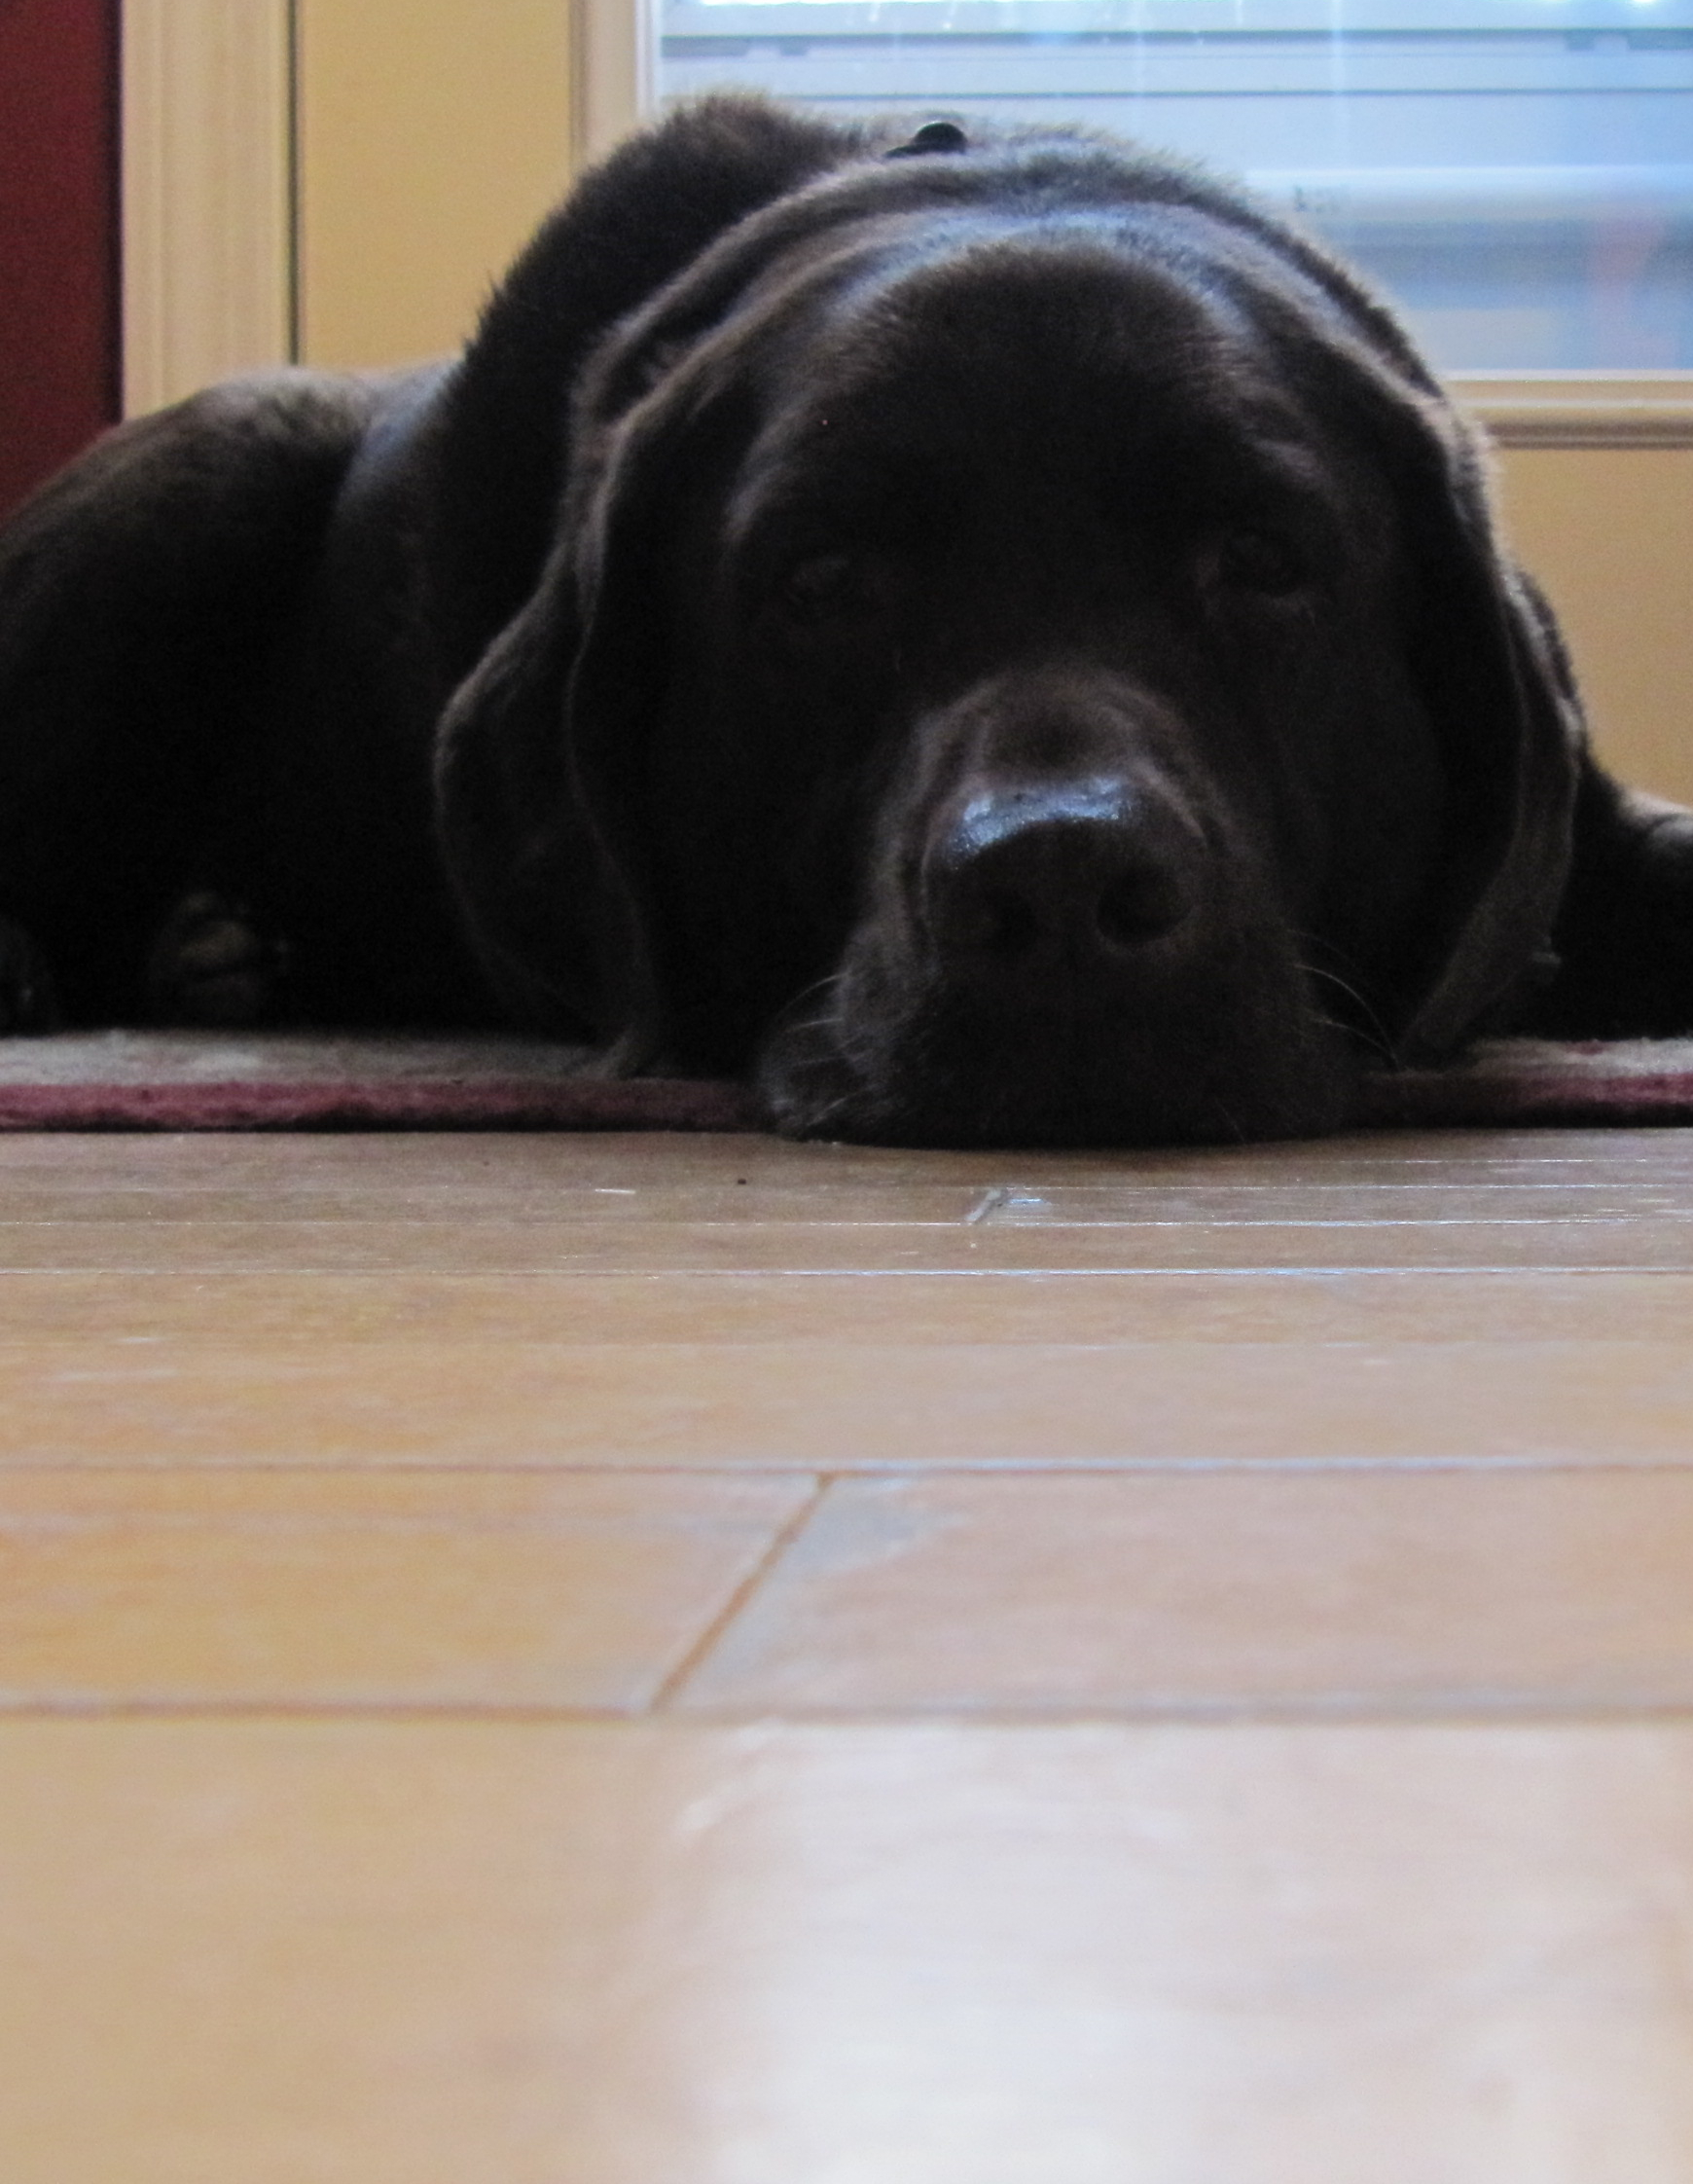
\includegraphics[width=.4\textwidth]{suzy_cover.png}}
  \quad
  \vcenteredhbox{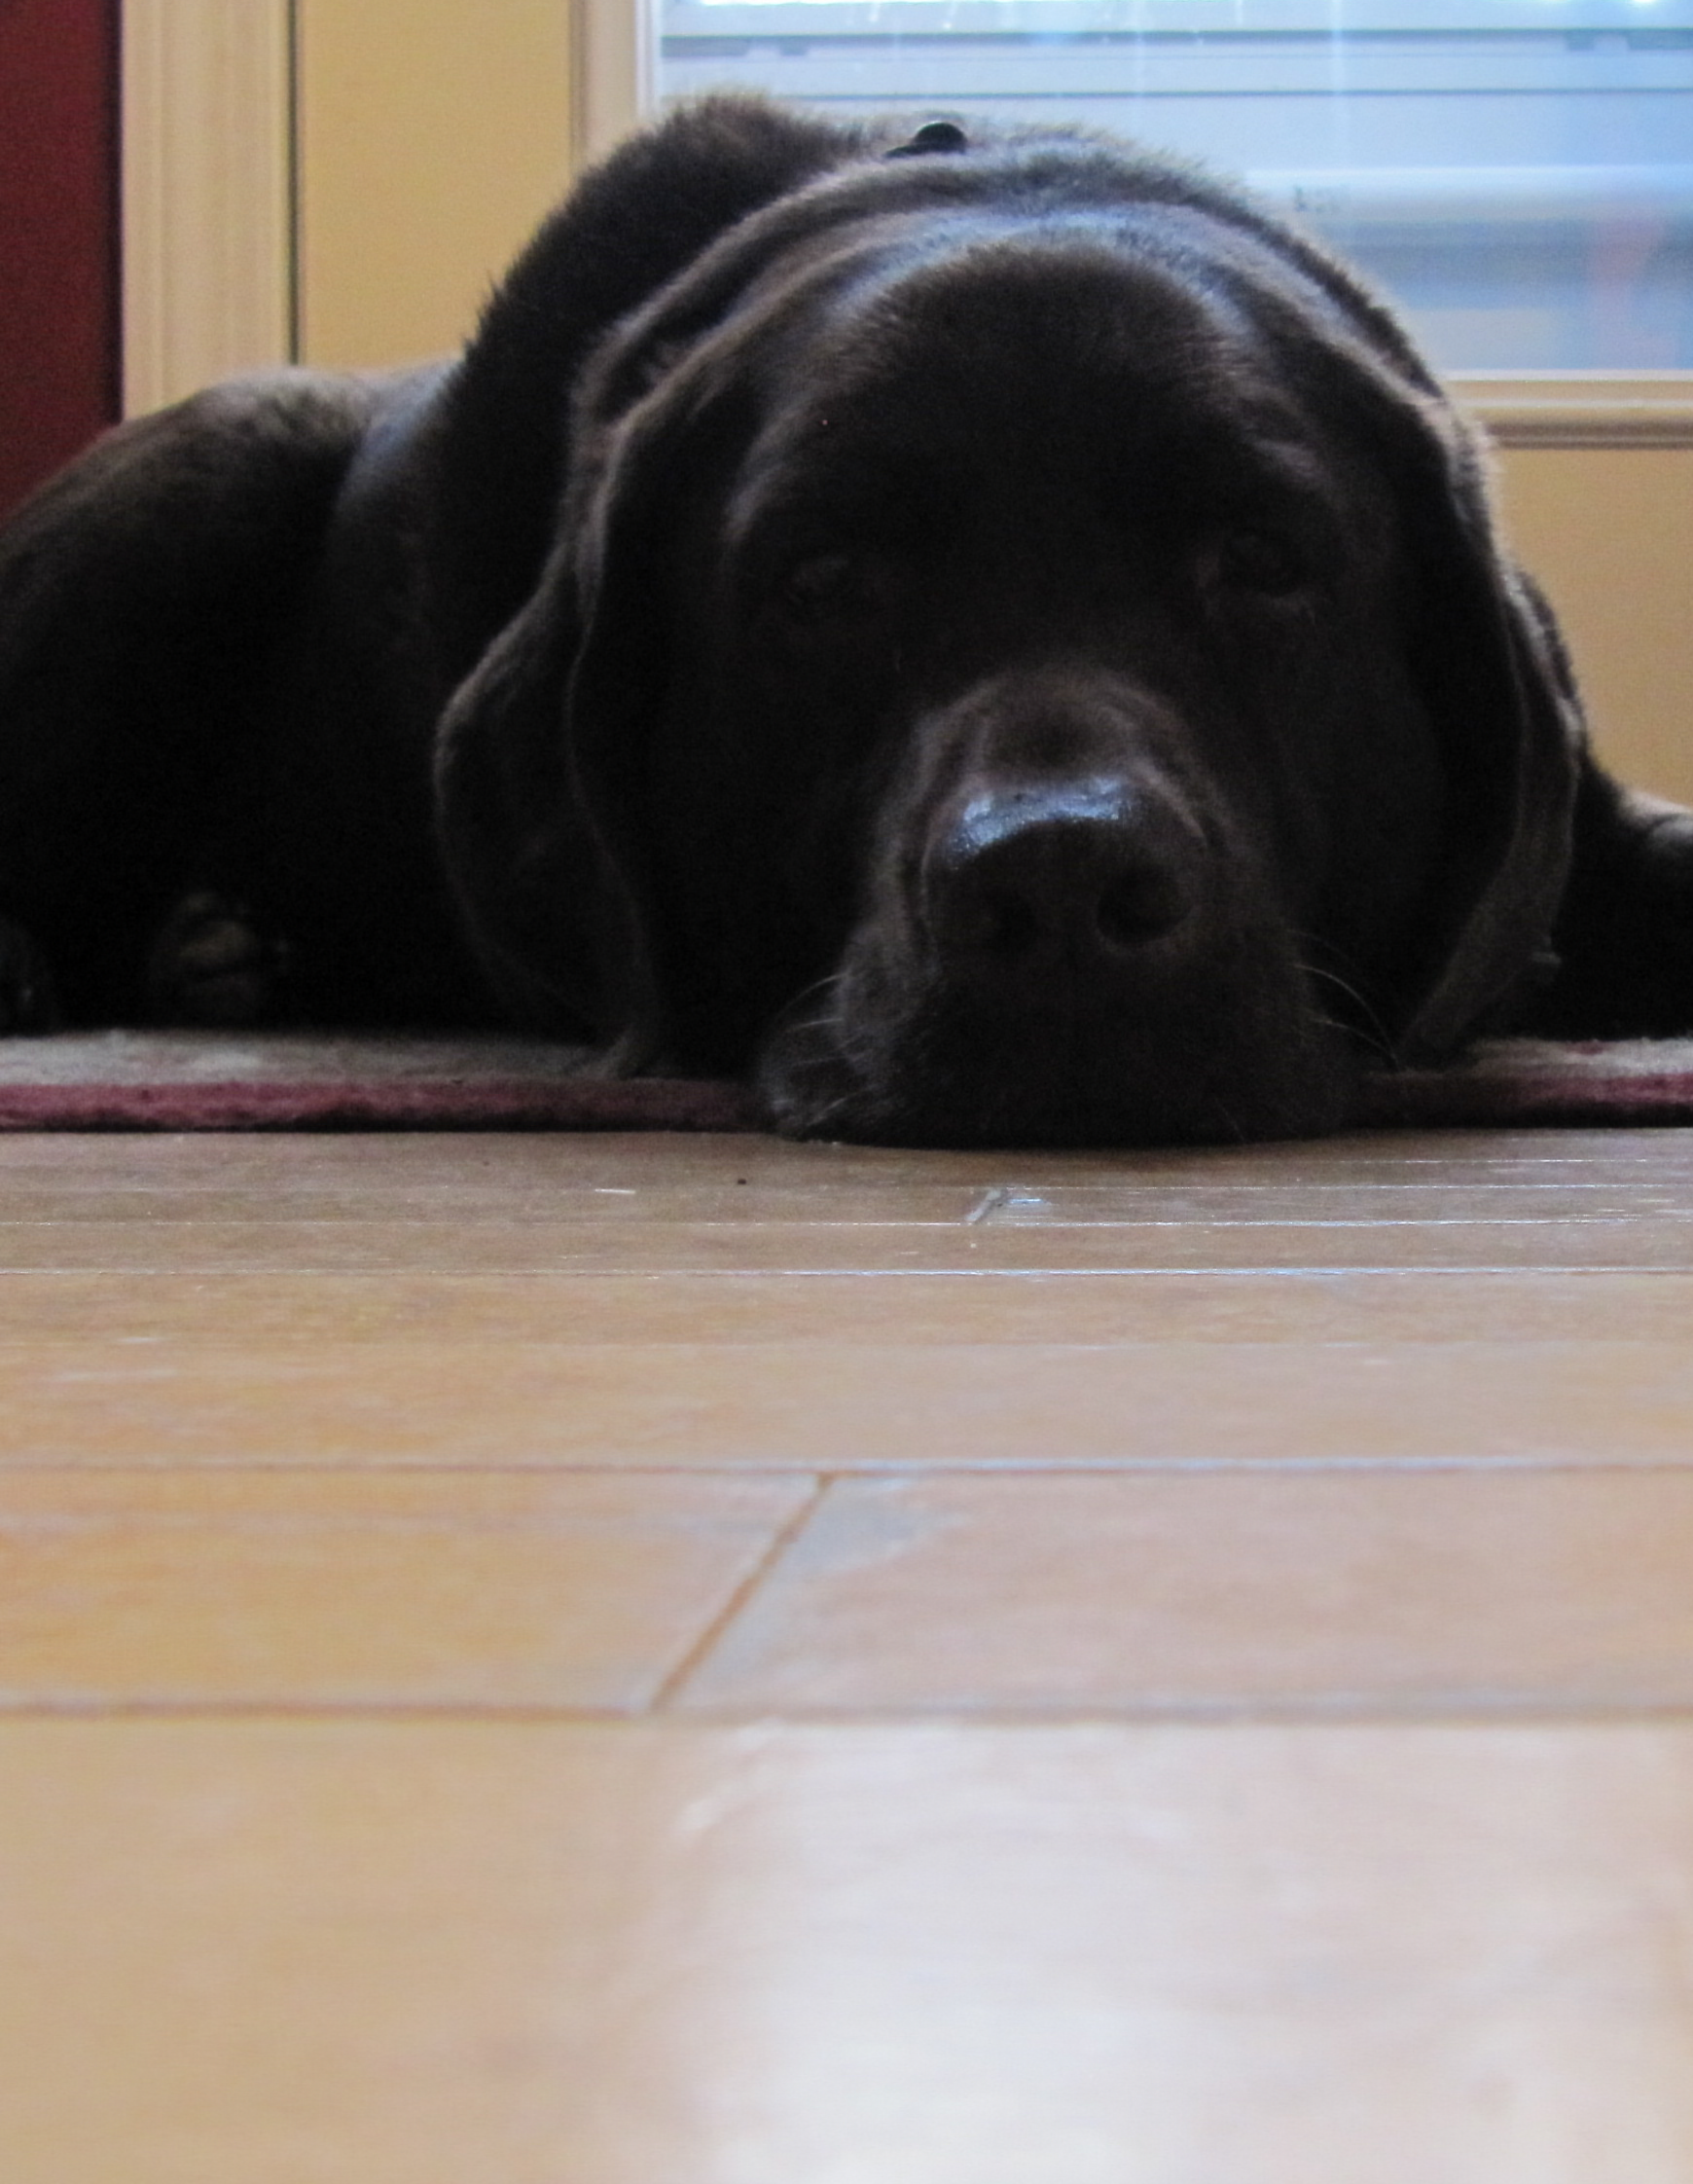
\includegraphics[width=.4\textwidth]{suzy_cover_squeezed.png}}
\end{center}



\section{Source of plot\_action.sage}

The \inlinecode{plot_circle_action}
routine that we call above takes the four entries of the $\nbyn{2}$
matrix and returns a list of graphics.
Other parameters are the number of colors, and a flag giving whether
to plot a full circle or whether to plot just the top half circle (this
is the default).

This routine determines the list of colors and 
calls a helper \inlinecode{color_circle_list}, 
given below, which returns a list of graphics.
Finally, this routine plots those graphics.
\lstinputlisting[firstline=38,lastline=48]{plot_action.sage}

The helper does the heavy lifting.
It produces a parametrized curve $(x(t),y(t))$, and uses \Sage's
\inlinecode{parametric_plot} function to get the resulting graphic.
\lstinputlisting[firstline=4,lastline=35]{plot_action.sage}
If this routine is plotting the upper half circle then it adds a
small empty circle at the end to show that the image of $(-1,0)$
is not part of the graph.

The global variable \inlinecode{CIRCLE_THICKNESS} sets the thickness of 
the plotted curve, in points (a printer's unit, here $1/72$~inch).
Similarly \inlinecode{DOT_SIZE} sets the size of the small empty circle.



\section{Source of img\_squeeze.sage}
We will use the Python Image Library for reading the figure.
The function
\inlinecode{img_squeeze}
takes three arguments, the names of the input and output functions, and
a real number between $0$ and $1$ which determines the percentage 
of the singular values to include in the sum before the cutoff.
\lstinputlisting[firstline=1,lastline=8]{img_squeeze.sage}

This function first brings the input data to a format where each
pixel is a triple 
$(\text{red}, \text{green},\text{blue})$ of integers that range from 
$0$ to~$255$.
It uses those numbers to gradually build 
three Python arrays \inlinecode{rd}, \inlinecode{gr},
and \inlinecode{bl}, which then initialize the 
three \Sage{} matrices \inlinecode{RD},
\inlinecode{GR}, and~\inlinecode{BL}.
\lstinputlisting[firstline=9,lastline=23]{img_squeeze.sage}

The next step finds the Singular Value Decomposition of those three.
Out of curiosity, we have a peek at the eight largest singular
values in the red matrix, the singular value where we make the cutoff,
and the eight smallest.
\lstinputlisting[firstline=24,lastline=36]{img_squeeze.sage}

Finally, for each matrix we compute the sum
$\sigma_1\cdot\vec{u}_1\trans{\vec{v}}_1+\sigma_2\cdot\vec{u}_2\trans{\vec{v}}_2
   +\cdots$
up through the cutoff index.
\lstinputlisting[firstline=37,lastline=56]{img_squeeze.sage}
The code asks for the transpose of the
\protect\inlinecode{U_RD.column(i)}, etc., which may seem to be a mistake.
Remember that \protect\Sage{} favors rows for vectors, so this is how we
make the $\vec{u}$ vector a column, while $\vec{v}$ is already a row.
Because of this operation on the vector, the first time you run this
code in a \protect\Sage{} session you may get a depreciation warning.

To finish, we put the data in the \path{.PNG} format and save it to 
disk.\lstinputlisting[firstline=57,lastline=66]{img_squeeze.sage}
This part of the routine function takes a very long time to run, in part because
the code is intended to be easy to read rather than fast.
Consequently, in the function source there are some status lines that
help convince a person executing the code that it is still working; 
those busy-work lines are left out of 
some of the earlier output listings.


\endinput


TODO:
1) mention Sage matrices are not mutable in matrix introduction.
Is mutable discussed in Intro?

2) Need int() fcns?  copy() fcn?